\documentclass[a4paper]{article}
\usepackage{fullpage, graphicx, array, url}

\begin{document}
	\title{Fundamentals of Information Visualisation - Coursework Report}
	\author{Harry Coupe, PSYHC5\\}
	\maketitle
	
	\section*{Initial Description of Data}
	The entire dataset is composed of information about Anime and the users of MyAnimeList who watch and review them. As written by the creator of the dataset "This dataset aims to be representative sample of internet otaku community for demographics analysis and trends inside this group. It contains information about users (gender, location, birth date etc.), about anime (airing date, genres, producer…) and anime lists".\\
	\\
	The data set as a whole contains:
	\begin{itemize}
		\item 302 675 unique users
		\item 302 573 of them with some demographic data
		\item 80 076 112 records in anime lists
		\item 46 358 322 of them have ratings
		\item 14 478 unique anime
	\end{itemize}
	For the purpose of my analysis I'll only be using the data based around the anime itself and not the user based data. The data set was acquired from: \textit{https://www.kaggle.com/azathoth42/myanimelist}.
	
	\pagebreak
	
	\section* {Initial Question 1 - Which years since 2000 have the most high rated anime?}
	To start for this question the dataset needed to be filtered down to relevant anime. The 3 parameters i set to meet this are: That the anime has completed airing that way ratings are for a completed product, More than 200 users have rated the anime to avoid anomalous entries and that the anime have an average score above 8.00. These 3 are what i deemed to be useable data points as a "high rated" anime. To do this i simply filtered the "anime" sheet into "anime\_filtered" using those 3 rules that were set.\\
	\\
	To make the data easier to work with a column for just year was needed. To achieve this by only using anime that was completed the final 4 characters of the "aired\_string" will always be the year it completed. Using the \texttt{substr} function and mutating it into a new column each anime entry now had a data point for what year it completed.\\
	\\
	After refining the data it needed to be sorted by year after 2000 and totalled by year. This was achieved using \texttt{group\_by} to organise the data by the year it completed and filtering that to entries with only years 2000 or greater. Then using the \texttt{dplyr} function \texttt{summarise} to total how man entries each year had and create the column \texttt{year\_total}.\\
	\\
	With the data finally prepared it is plotted using a \texttt{ggplot2 geom\_bar} with the colour filling mapped the to increasing year.\\
	\noindent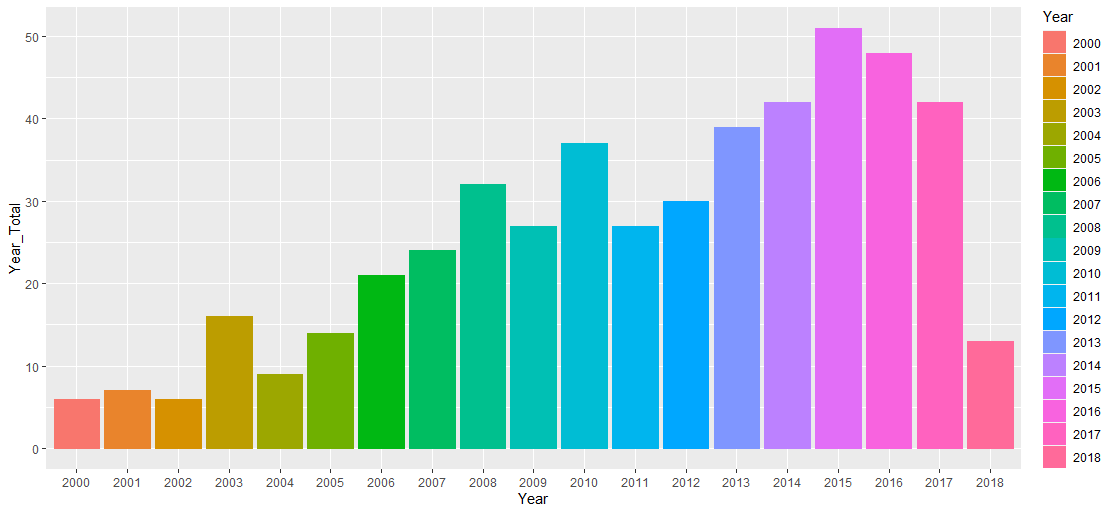
\includegraphics[scale=0.55]{TopAnimeByYear.png}
	
	\pagebreak
	
	\subsection*{Sub-question: For the top 5 years what are the top 10 genres within them?}
	Once the data was visualised for the initial question I wanted to know which genres were the most popular in the top 5 years from this data set. To be able to plot this data it needs to be further refined. To get the data in the required format I once again started the the "anime\_filtered" sheet. From there the data is \texttt{group\_by}'d with the 2 relevant columns, year and genre. Then the \texttt{Tidyr} function \texttt{separate\_rows} is used to split each anime's list of genre tags into their own individual data entries. So it will take "Comedy, School, Shounen" and split them into 3 separate entries for the same anime. Then that data is summarised into a \texttt{Total\_Genre} column to count how many high rated anime their are for each genre. Finally that data is subset to the years 2013 - 2017 which are the top 5 years found from the previous visualisation.\\
	\\
	For the visualisation I wanted to use a radar graph for each year so to save on constantly typing out the same code I made a custom function to make all of the radar graphs from and will take the name of the graph and the colour to be used for the graph as arguments.\\
	\\
	Finally when it comes to plotting each graph i subset the data again to the desired year, arrange the \texttt{Total\_Genre} column descending and head the top 10 results from that data to plot in each radar.\\
	
	\begin{figure}[!htb]
		\minipage{0.32\textwidth}
		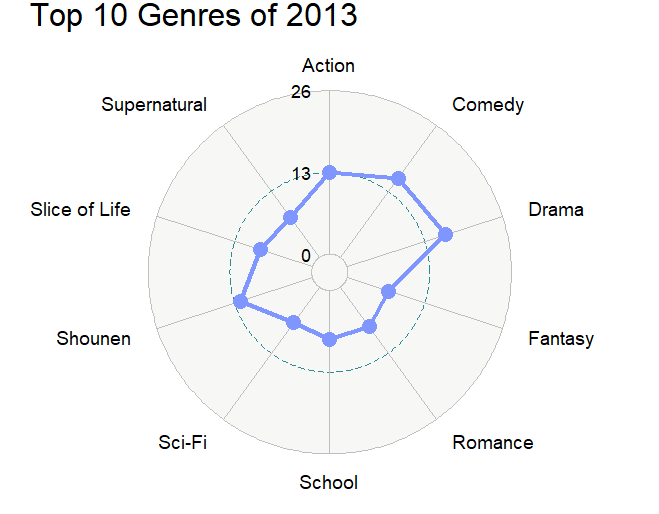
\includegraphics[width=\linewidth]{2013Radar.png}
		\endminipage\hfill
		\minipage{0.32\textwidth}
		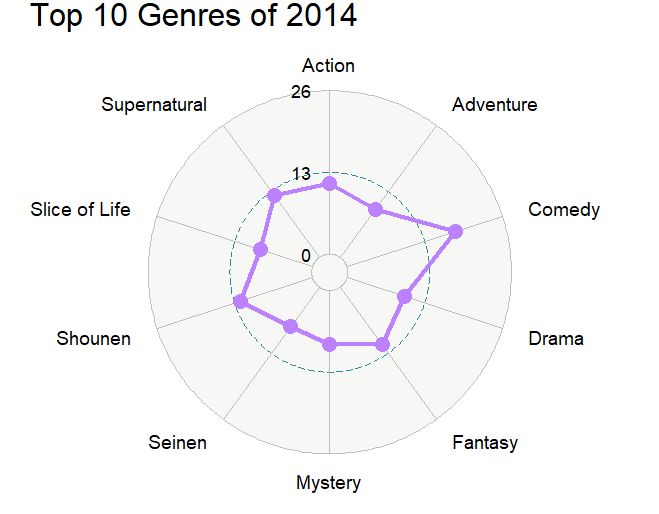
\includegraphics[width=\linewidth]{2014Radar.png}
		\endminipage\hfill
		\minipage{0.32\textwidth}%
		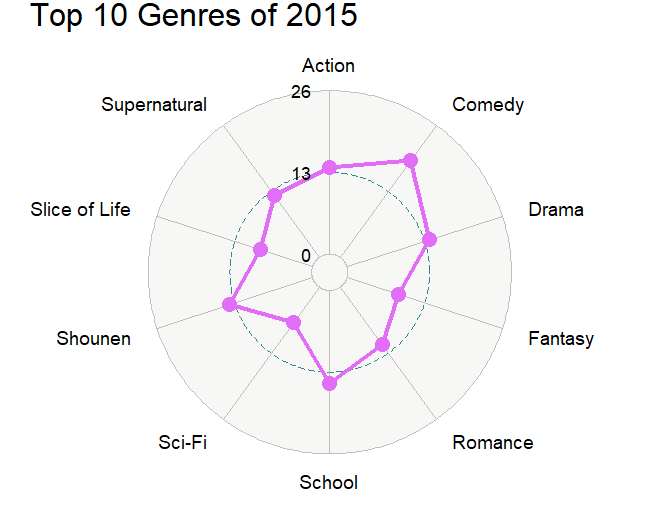
\includegraphics[width=\linewidth]{2015Radar.png}
		\endminipage
	\end{figure}
	\begin{figure}[!htb]
	\minipage{0.32\textwidth}
		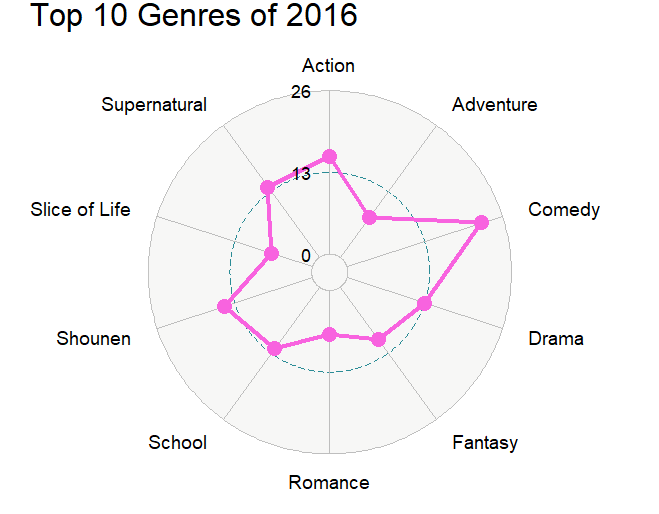
\includegraphics[width=\linewidth]{2016Radar.png}
		\endminipage\hfill
		\minipage{0.32\textwidth}
		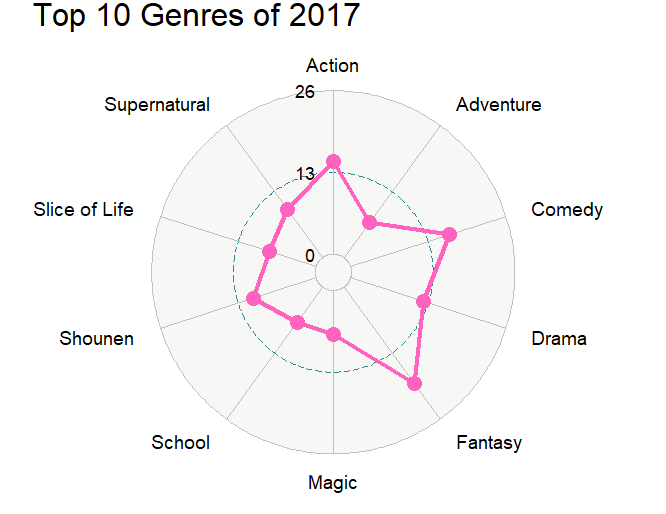
\includegraphics[width=\linewidth]{2017Radar.png}
		\endminipage
	\end{figure}

	\pagebreak
	
	\section* {Initial Question 2 - Which of the source materials has the most high rated anime?}	
	After seeing what years and genres had been popular the next area of the dataset that stood out as interesting was the source material that each anime were based on. So from this I wanted to plot which source material had the most high rated anime.\\
	\\
	Similar to previous visualisations starting with "anime\_filtered" i group by source, filter to later than 2000 then summarise into a total column for each source so the data is easy to plot. Then because there are fewer data points i plot this bar graph with the \texttt{scale\_fill\_brewer} palette "Set3" to make sure it looks different from the previous graphs.\\
	\noindent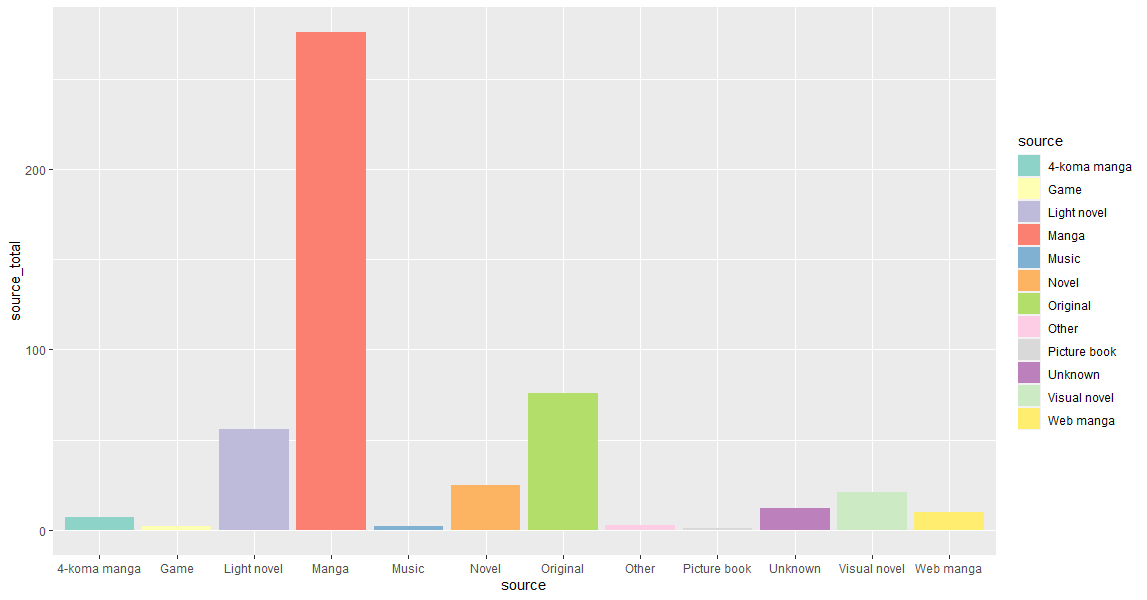
\includegraphics[scale=0.60]{TopAnimeBySource.png}
	
	\pagebreak
	
	\subsection*{Sub-question: For the most popular source, manga, what type of anime is most commonly high rated?}
	After seeing the previous visualisation it's clear just how much more popular manga is as a source so wanted to do a deeper dive into what makes up manga as a source for anime. So to see what makes up manga sourced anime I decided to see what "type" of anime is most often highly rated for anything based on a manga. By type I mean whether it was a TV show or movie or spin off etc.\\
	The data cleaning and transformation for this visualisation is mostly the same to the last plot bar instead of grouping by source its by type. Then filtering the results of that to include post 2000s anime that are only based on manga. Again, because the dataset is a little smaller again I decide to plot with the palette "Dark2" to ensure visualisations are clearly distinguishable at a glance.\\
	\noindent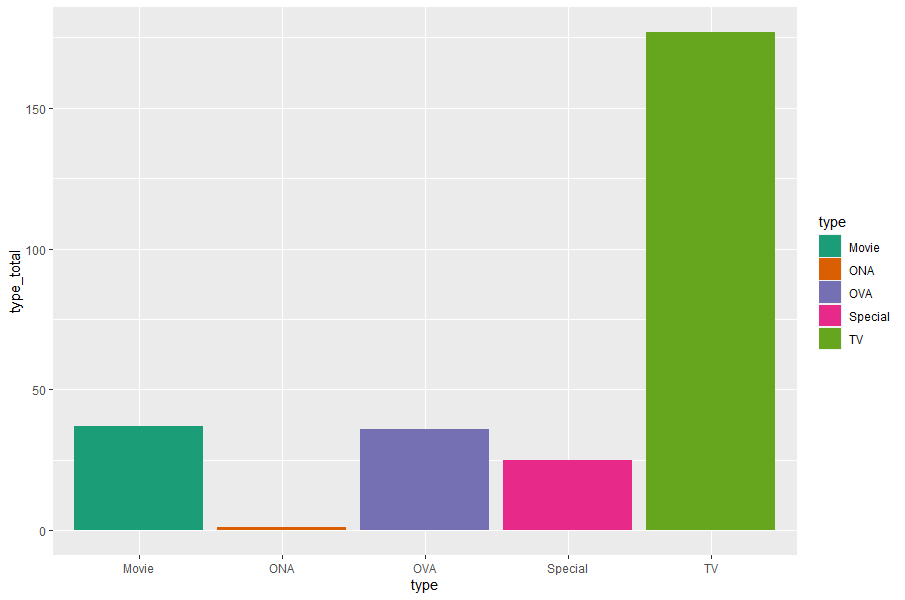
\includegraphics[scale=0.60]{TopAnimeTypeByManga.png}
	
	\pagebreak
	  
	\subsection*{Sub-question: The highest rating of an anime of each source material}
	Finally, for this section I wanted to see if the popularity of manga as a source affect its peak score compared to every other source material. This data like all of the rest starts from "anime\_filtered", grouping by source and filtering to post 2000s. After that I use the \texttt{dplyr} function \texttt{arrange} to sort the data by source and then within that sort the scores descending so the top of each source is the highest score. Then using the \texttt{first} function inside of \texttt{summarise} to have each source collapsed down to just its highest score.\\
	\noindent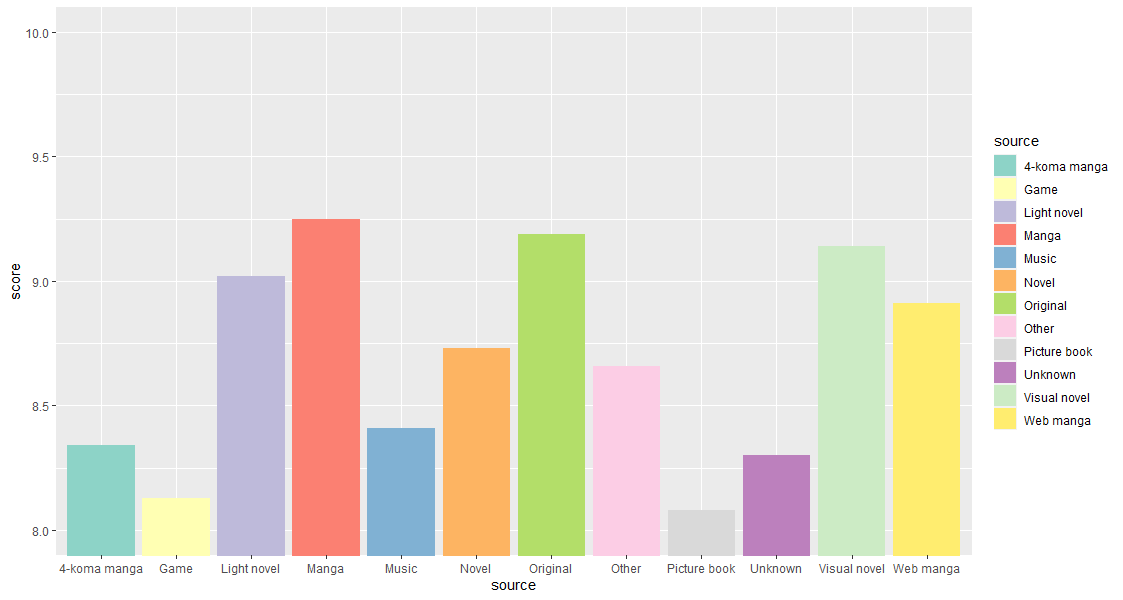
\includegraphics[scale=0.60]{HighestRatingBySource.png}
	
	\pagebreak
	
	\section* {Initial Question 3 - Which years since 2000 have the most bad anime?}
	After spending 2 questions looking at what that dataset says about good anime I wanted to see the opposite and do some diving into data behind bad anime. I quantified this to be an anime that is scored by more than 200 users, has a score greater at 0.00 but less than or equal to 5.00 and has finished airing. Using these parameters and mutating the year column into it again the same as with the first sheet I made the "bad\_anime\_filtered" sheet.\\
	\\
	Apply a filter for anime after 2000 and grouping by year and summarising to total how many bad anime there are in each year then plotting that in a bar graph.\\ 
	\noindent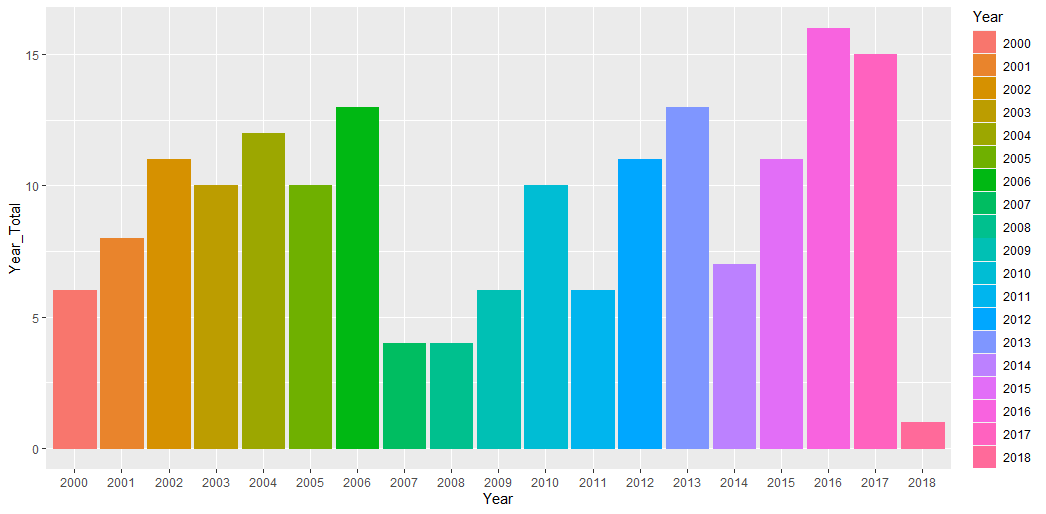
\includegraphics[scale=0.60]{BadAnimeByYear.png}
	
	\pagebreak
	
	\subsection*{Sub-question: Which genres have the most bad anime?}
	As well as years I wanted to see what genres also have the most bad anime. Using the "bad\_anime\_filtered" sheet and grouping by year, separating the rows and summarising so each anime has an entry per genre tag. Also decided to filter genres to any with more than 2 bad anime to clear out the clutter in the visualisation. This is then plotted on a bar graph.\\
	\noindent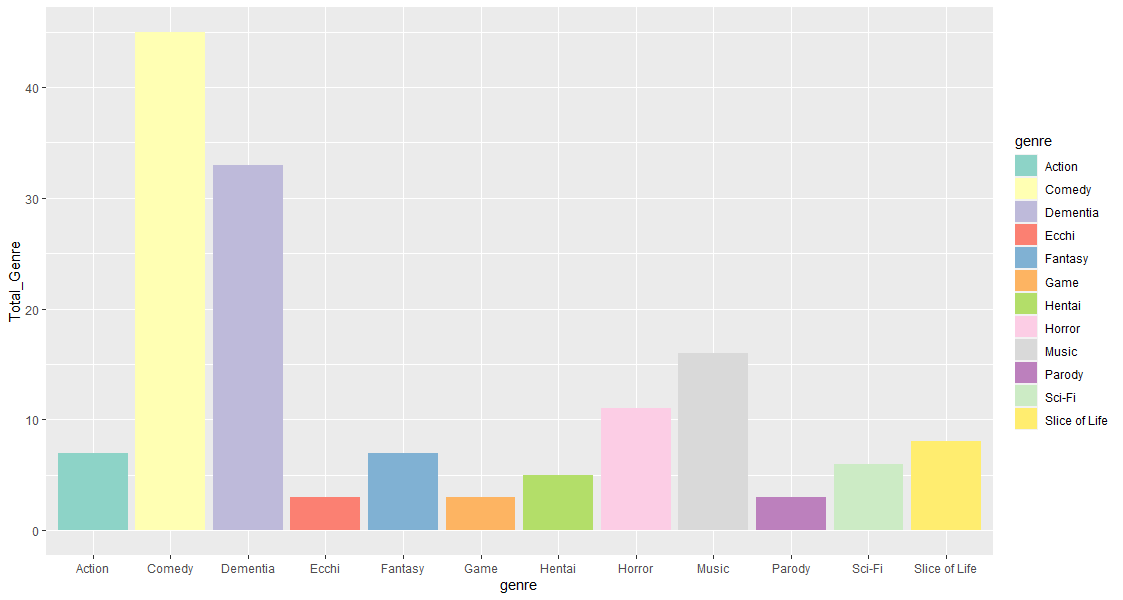
\includegraphics[scale=0.60]{BadAnimeByGenre.png}
	
		
	\section* {Design \& Reflections}
	A lot of my designs came out to being bar graphs purely because it was the most efficient way of answering the questions I wanted to ask of the data set and trying to come up with questions that didn't just end in a bar graph proved to be a lot more challenging than anticipated. I tried to make each bar graph a little more distinct using different colour palettes but again proves challenging when 6/7 visualisations are bar graphs.\\
	\\
	Whilst I'm not disappointed with the visualisations I came out with had I had a lot more prior experience with javascript I would've liked to use Chart.js to make interactive versions of my visualisations showing, for example, in my initial question 1 visualisation when each bar is mouseovered would show the top 5 ranked anime of that year and the cover for first place. But a lack of experience and time left me with just the ideas for these interactive visualisations.\\
	\\
	
\end{document}